\subsection{Posredovanje u zapo\v sljavanju}

Poslodavac \v zeli da zaposli radnika preko NSZ. On dolazi u slu\v zbu i na \v salteru mu ka\v zu da moraju da ga registruju u njihovu bazu poslodavaca. Poslodavac se registruje i nakon toga objavljuje oglas za nepopunjeno radno mesto u njegovoj kompaniji. Daje opis radnog mesta i uslove koje radnik mora da ispuni. Nakon toga poslodavac zapo\v sljava radnika i pravi se izve\v staj o realizaciji konkursa. 


\subsubsection{Slu\v caj upotrebe: Registracija poslodavca}

\noindent Učesnici: Poslodavac, šalterski službenik.
\\
\\ Preduslovi: Poslodavac ima ličnu kartu.
\\
\\ Postuslovi: Poslodavac je uspešno registrovan.
\\
\\ Glavni tok:
\begin{enumerate}
\item Poslodavac prilazi automatu i bira opciju ''Registracije i verifikacije kompanije''.
	\item Automat bele\v zi da je opcija ''Registracije i verifikacije kompanije'' odabrana, ra\v cuna naredni broj u redu \v cekanja za tu opciju, i \v stampa papir sa brojem.
	\item Poslodavac uzima broj i \v ceka svoj red.
	\item Kada do\dj e na red, poslodavac prilazi \v salteru i zahteva od \v SS da ga registruje u sistemu.
	\item \v SS tra\v zi od poslodavca da mu preda li\v cnu kartu.
	\item Poslodavac predaje ličnu kartu. 
	\item \v SS daje poslodavcu formular za prijavu.
    \item Poslodavac popunjava prijavu, a zatim je vra\v ca SS-u.
	\item \v SS unosi informacije sa prijave u sistem.
	\item \v SS vra\' ca ličnu kartu poslodavcu.
	\item Prelazi se na slu\v caj upotrebe \ref{su: razgovor sa poslodavcem}.
\end{enumerate}



\subsubsection{Slu\v caj upotrebe: Objava konkursa}
\label{su: razgovor sa poslodavcem}

\noindent Učesnici: Poslodavac, savetnik za rad sa poslodavcima (u daljem tekstu savetnik).
\\
\\ Preduslovi: Poslodavac ima ličnu kartu i registrovan je u sistem.
\\
\\ Postuslovi: Konkurs je objavljen.
\\
\\ Glavni tok:
\begin{enumerate}
\item Poslodavac dolazi kod savetnika u kancelariju i saopštava mu da želi da zaposli radnika.
\item Savetnik traži od poslodavca da mu da ličnu kartu.
\item Poslodavac daje savetniku ličnu kartu.
\item Savetnik na osnovu podataka sa lične karte traži poslodavca u sistemu.
\item Savetnik traži od poslodavca da navede detalje o radnom mestu.
\item Poslodavac saopštava savetniku detalje o radnom mestu.
\item Savetnik unosi informacije u sistem.
\item Savetnik daje poslodavcu da popuni formular o konkursu na radno mesto.
\item Poslodavac popunjava formular, a zatim ga vraća savetniku.
\item Savetnik prosleđuje informacije svim nezaposlenima koji zadovoljavaju kriterijume iz konkursa. Slučaj upotrebe se završava.
\end{enumerate}

\subsubsection{Slu\v caj upotrebe: Realizacija konkursa}

\noindent U\v cesnici: Poslodavac, savetnik za rad sa poslodavcima (u daljem tekstu savetnik).
\\
\\ Preduslovi: Poslodavac ima dokaz o zapošljavanju nezaposlenog lica.
\\
\\ Postuslovi: Poslodavac je zaposlio nezaposleno lice i kompletiran je izve\v staj o realizaciji konkursa.
\\
\\ Glavni tok:
\begin{enumerate}
\item Poslodavac dolazi kod savetnika u kancelariju i predaje mu dokaz o zapošljavanju lica sa evidencije NSZ.
\item Savetnik pronalazi nezaposleno lice u sistemu i skida ga sa evidencije.
\item Savetnik daje poslodavcu da popuni formu o realizaciji konkursa.
\item Poslodavac popunjava  formu o realizaciji konkursa i predaje je savetniku.
\item Savetnik realizuje konkurs i uklanja ga iz sistema.
\item Savetnik vraća dokaz o zapošljavanju  poslodavcu, slučaj upotrebe se završava.
\end{enumerate}

\begin{mylandscape}
	\subsubsection{BPMN dijagrami}
	
	\begin{figure}[H]
		\centering
		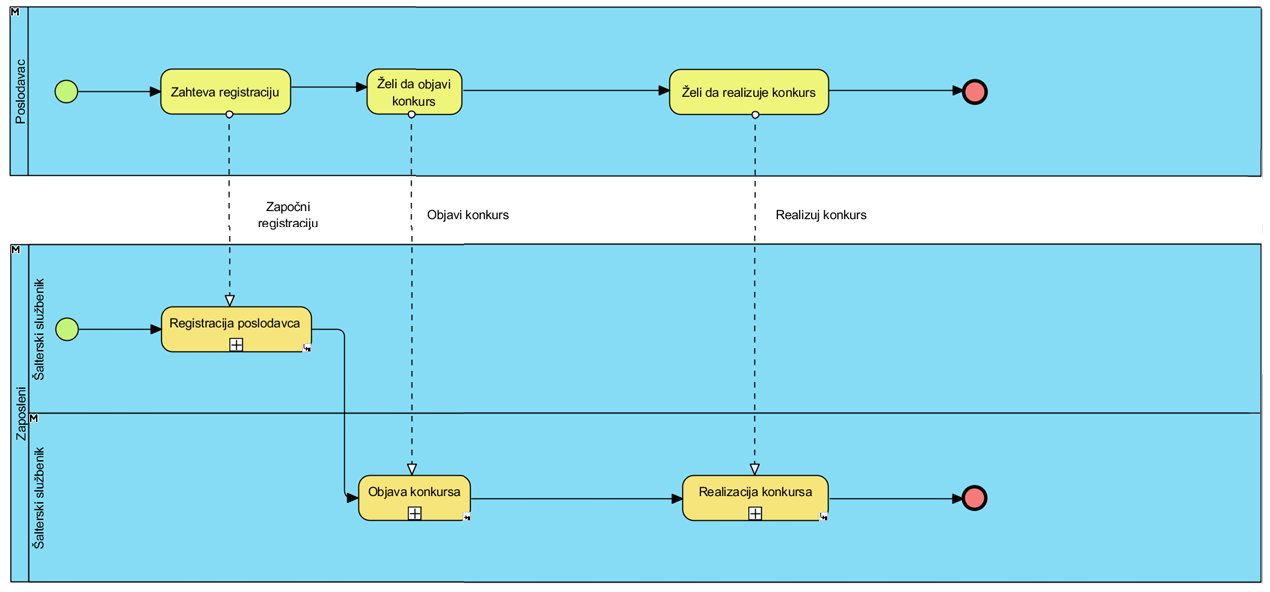
\includegraphics[width=0.7\paperwidth]{dijagrami/bpmn-dijagrami/bpmn-7.png}
		\caption{BPMN dijagram procesa ''Posredovanje u zapo\v sljavanju''.}
		\label{bpmnd: posredovanje u zaposljavanju}
	\end{figure}
	
	\newpage
	
	\begin{figure}[H]
		\centering
		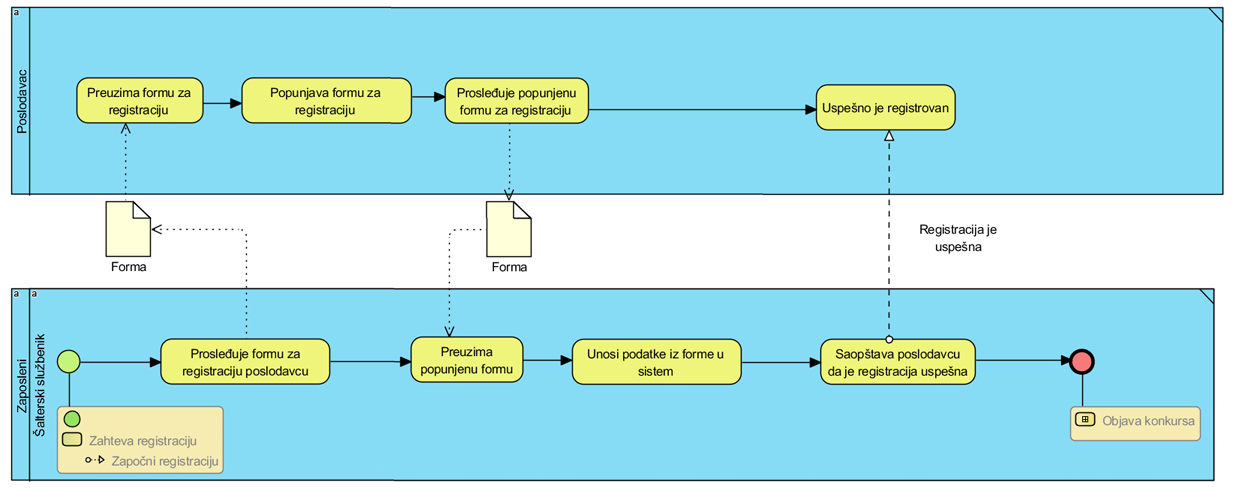
\includegraphics[width=0.7\paperwidth]{dijagrami/bpmn-dijagrami/bpmn-8.png}
		\caption{BPMN dijagram potprocesa ''Registracija poslodavca'' procesa ''Posredovanje u zapo\v sljavanju'' (\ref{bpmnd: posredovanje u zaposljavanju}).}
	\end{figure}

	\newpage
	
	\begin{figure}[H]
		\centering
		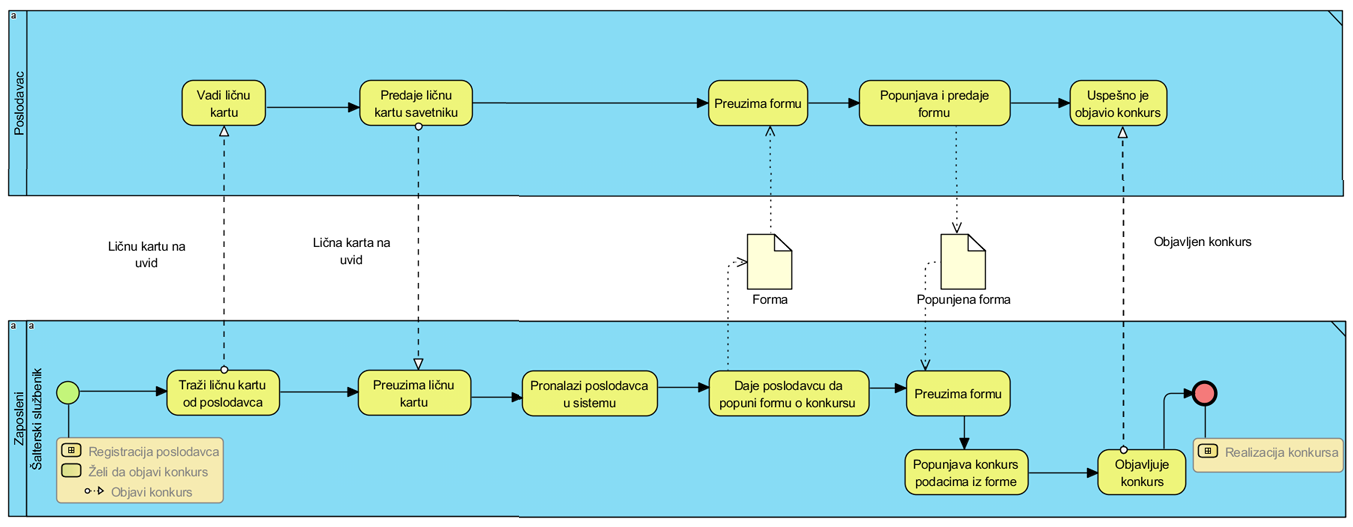
\includegraphics[width=0.7\paperwidth]{dijagrami/bpmn-dijagrami/bpmn-9.png}
		\caption{BPMN dijagram potprocesa ''Objava konkursa'' procesa ''Posredovanje u zapo\v sljavanju'' (\ref{bpmnd: posredovanje u zaposljavanju}).}
	\end{figure}

	\newpage
	
	\begin{figure}[H]
		\centering
		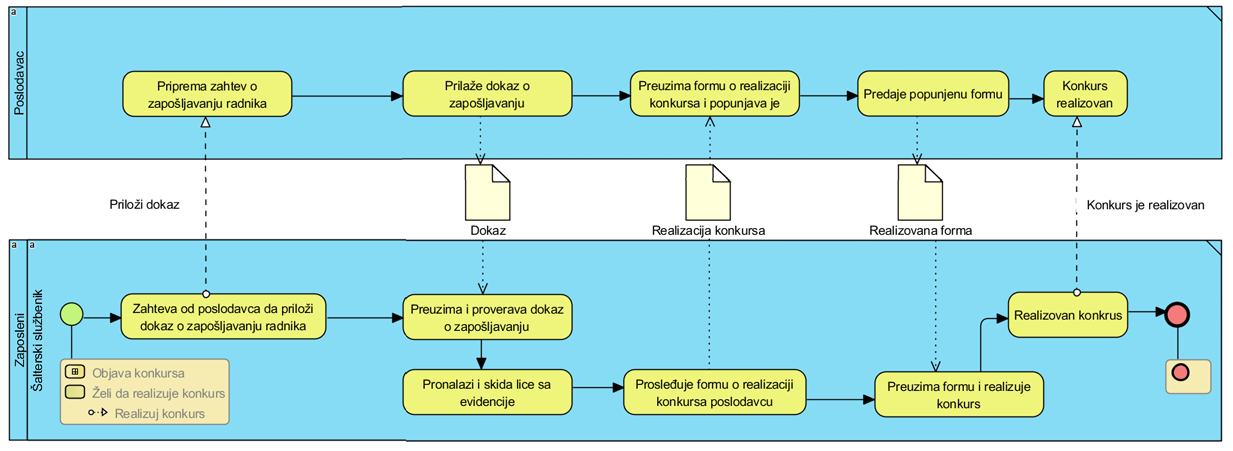
\includegraphics[width=0.7\paperwidth]{dijagrami/bpmn-dijagrami/bpmn-10.png}
		\caption{BPMN dijagram potprocesa ''Realizacija konkursa'' procesa ''Posredovanje u zapo\v sljavanju'' (\ref{bpmnd: posredovanje u zaposljavanju}).}
	\end{figure}
	
\end{mylandscape}